% =============================================================================
% INITIAL DRAFT -- Paper B (Journal of Supercomputing)
%
% Generated as part of the two-paper research plan in ../PLAN.md. Uses a
% portable `article` preamble (matching docs/CALL_FOR_PAPERS.tex) as a stand-in
% for the official Springer Nature `sn-jnl` class, which should be substituted
% before submission (see PLAN.md sec. 8). The RTX 4070 tables/figures in
% Section 7.1 are REAL, already-measured results reused as an interim
% reference platform. The cross-hardware Jetson Nano / Xilinx ZCU102 tables in
% Section 7.2 are MOCK PLACEHOLDERS (no such hardware has been benchmarked
% yet) -- see the draft-status banner and PLAN.md sec. 5 for the labeling
% convention.
% =============================================================================
\documentclass[11pt,a4paper]{article}

\usepackage[utf8]{inputenc}
\usepackage[T1]{fontenc}
\usepackage{geometry}
\geometry{top=1in, bottom=1in, left=1in, right=1in}
\usepackage{amsmath}
\usepackage{amssymb}
\usepackage{microtype}
\usepackage{graphicx}
\usepackage{booktabs}
\usepackage{multirow}
\usepackage{xcolor}
\usepackage{cite}
\usepackage{hyperref}

\graphicspath{{../../docs/plots/}}

\hypersetup{
    colorlinks=true,
    linkcolor=blue,
    filecolor=magenta,
    urlcolor=cyan,
    citecolor=blue,
}

% ---- Mock-data / placeholder conventions (see PLAN.md sec. 5) ----------------
\newcommand{\mocknote}{{\footnotesize\color{red!60!black}\textit{(Mock data --- placeholder pending real edge-hardware benchmarking; see Section~\ref{sec:reproducibility}.)}}}
\newcommand{\realnote}{{\footnotesize\color{blue!50!black}\textit{(Real, already-measured interim reference-platform results.)}}}
\newcommand{\figureplaceholder}[2]{%
\begin{figure}[ht]
\centering
\setlength{\fboxsep}{0pt}
\fbox{\begin{minipage}[c][0.28\textheight][c]{0.85\textwidth}
\centering
{\color{gray}\rule{0.8\textwidth}{0.4pt}}\\[0.8em]
{\bfseries\color{gray!60!black} FIGURE PLACEHOLDER}\\[0.4em]
{\color{gray!70!black}\itshape pending edge-hardware benchmark}\\[0.8em]
{\color{gray}\rule{0.8\textwidth}{0.4pt}}
\end{minipage}}
\caption{#2}
\label{fig:#1}
\end{figure}}

\title{\textbf{Optimizing Self-Supervised Power-Converter Anomaly Detectors for Edge AI: A GPU-Embedded (Jetson Nano) versus FPGA-Embedded (Xilinx Zynq UltraScale+) Comparison}}

\author{
    \textbf{Ignacio Martin-Salinas}, \textbf{Jose A. Belloch}, \textbf{Cristina Fernandez} \\
    \small Depto. de Tecnolog\'{i}a Electr\'{o}nica, Universidad Carlos III de Madrid, Madrid, Spain
}
\date{}

\begin{document}
\maketitle

\begin{center}
\fcolorbox{red!60!black}{red!5}{\begin{minipage}{0.92\textwidth}
\small\textbf{Draft status.} This is an \emph{initial draft} scaffolding the manuscript
structure and benchmarking methodology. Section~\ref{sec:results-rtx} (RTX~4070 interim
platform) reports \textbf{real, already-measured} results. Section~\ref{sec:results-edge}
(Jetson Nano / Xilinx ZCU102 cross-hardware comparison) is entirely \textbf{mock
placeholder data} -- no edge hardware has been benchmarked yet. See
Section~\ref{sec:reproducibility} for the exact commands to close this gap.
\end{minipage}}
\end{center}

\begin{abstract}
Real-time condition monitoring of power electronic converters increasingly demands
inference at the sensor edge rather than on a networked workstation, yet the
computational cost of modern deep anomaly detectors is rarely evaluated on the
resource-constrained hardware such systems must ultimately run on. This paper studies
the systems-level optimization and edge deployment of a self-supervised anomaly
detection pipeline for power-converter frequency-response signatures (the modeling
methodology itself is presented in a companion submission to \emph{Mathematical Methods
in the Applied Sciences}), focusing on a uniform quantization and export pipeline
(TensorFlow Lite, ONNX Runtime, NVIDIA TensorRT, and Xilinx Vitis AI) and a
head-to-head comparison of a GPU-embedded target (NVIDIA Jetson Nano) against an
FPGA-embedded, DPU-based target (Xilinx Zynq UltraScale+ MPSoC, ZCU102/ZCU104). On an
interim RTX~4070 workstation-GPU reference platform, our existing pipeline already
collapses batch-1 inference latency from a $19.75\text{ ms}$ Keras FP32 GPU baseline to
$0.499\text{ ms}$ under TensorRT FP16 (a $39\times$ speedup) at near-lossless
classification fidelity (ROC-AUC $>0.98$). Cross-hardware results on Jetson Nano and
Xilinx ZCU102/ZCU104 --- including latency, memory footprint, and energy per inference
--- are reported as placeholders pending on-device benchmarking (\textbf{[MOCK]}
throughout Section~\ref{sec:results-edge}) and are the focus of the ongoing experimental
campaign described in Section~\ref{sec:reproducibility}.
\end{abstract}

\noindent\textbf{Keywords:} Edge Computing; Model Quantization; TensorRT; Vitis AI;
FPGA; Jetson Nano; Power Electronics; Anomaly Detection; High-Performance Computing

\section{Introduction}
\label{sec:intro}

Power electronic converters are safety- and mission-critical components in aerospace,
electric-vehicle, and grid infrastructure, where undetected parametric degradation can
precede catastrophic failure~\cite{idrisov2025digitaltwin,liu2022review}. A companion
paper~\cite{darban2023carla} details a self-supervised, contrastive deep-learning
pipeline that detects such degradation from a converter's frequency-response (Bode)
signature; this paper takes that trained pipeline as a fixed workload and asks a
systems question: \emph{what does it cost, in latency, memory, and energy, to run this
class of model in real time on the resource-constrained hardware co-located with the
converter, and how does that cost compare across fundamentally different edge-compute
architectures?}

Two edge targets are of particular interest because they represent the two dominant
philosophies for embedded AI inference: a small \textbf{GPU-embedded} system-on-module
(NVIDIA Jetson Nano, reusing the CUDA/TensorRT software stack already validated on a
workstation GPU) and an \textbf{FPGA-embedded}, dataflow-oriented accelerator (Xilinx
Zynq UltraScale+ MPSoC, via the Vitis AI Deep-Learning Processing Unit, or DPU). These
represent, respectively, a flexible but power-hungrier software-programmable path and a
statically compiled, potentially more deterministic and power-efficient hardware
dataflow path. Prior work on edge deployment of power-electronics anomaly detectors has
emphasized model accuracy and self-commissioning aspects~\cite{gomez2023selfcommissioning,beattie2022robust}
more than a rigorous, uniform cross-hardware latency/memory/energy benchmark; general
surveys of neural-network accelerators and quantization
techniques~\cite{sze2017efficient,gholami2021quantsurvey,jacob2018quantization} and
tiny-ML benchmarking suites~\cite{banbury2021mlperftiny} provide methodology but are not
specific to this workload or to the GPU-vs-FPGA embedded comparison studied here.

This paper's contributions are:
\begin{enumerate}
    \item A uniform quantization and export pipeline covering TensorFlow Lite (dynamic,
    float16, INT8), ONNX Runtime, NVIDIA TensorRT (FP32/FP16/INT8), and Xilinx Vitis AI
    (INT8, DPU-compiled), applied to the same trained anomaly-detection model
    (Section~\ref{sec:pipeline}).
    \item A single-sample (batch-1), warm-up-controlled timing protocol applied
    identically across every backend and, in this extended study, across every target
    device (Section~\ref{sec:methodology}).
    \item An interim reference measurement of the full pipeline on an RTX~4070
    workstation GPU (Section~\ref{sec:results-rtx}, real data), establishing the
    achievable latency/fidelity envelope before edge-hardware constraints are applied.
    \item A head-to-head GPU-embedded (Jetson Nano) vs.\ FPGA-embedded (Xilinx Zynq
    UltraScale+) comparison across latency, memory, model size, classification fidelity
    retention, and energy per inference (Section~\ref{sec:results-edge}, placeholders
    pending the benchmarking campaign of Section~\ref{sec:reproducibility}).
\end{enumerate}

\section{Related Work}
\label{sec:related}

\textbf{Quantization and efficient inference.} Integer-arithmetic quantization schemes
trade numerical precision for latency, memory, and energy
reductions~\cite{jacob2018quantization,gholami2021quantsurvey}; efficient deep-network
inference more broadly has been surveyed extensively~\cite{sze2017efficient}. Standard
ML systems (Keras~\cite{chollet2015keras}, TensorFlow~\cite{abadi2016tensorflow},
ONNX~\cite{bai2019onnx}, NVIDIA TensorRT~\cite{nvidia2020tensorrt}) provide the export
and runtime layers this paper builds on.

\textbf{Embedded/edge AI benchmarking.} Benchmark suites such as MLPerf
Tiny~\cite{banbury2021mlperftiny} standardize latency/energy measurement methodology for
microcontroller- and SoC-class devices; this paper adopts a comparable uniform-protocol
philosophy (Section~\ref{sec:methodology}) but applies it to a specific, real
power-electronics workload rather than a generic benchmark model.

\textbf{GPU-embedded vs.\ FPGA-embedded inference.} NVIDIA Jetson-class modules provide a
CUDA/TensorRT software stack largely compatible with workstation-GPU development,
whereas Xilinx/AMD Vitis AI compiles models to a statically scheduled DPU bitstream
running on programmable logic. Both paths are used throughout the embedded-ML
literature, but a direct, uniform-protocol comparison of the two on the same trained
anomaly-detection model is --- to our knowledge, and within the scope of this
project --- not yet available; closing that gap is this paper's systems contribution.

\textbf{Power electronics condition monitoring at the edge.} Self-commissioning and
edge-oriented anomaly detection for power electronics has been studied
directly~\cite{gomez2023selfcommissioning} and via digital-twin
approaches~\cite{idrisov2025digitaltwin}, generally without a systematic multi-backend,
multi-hardware performance-engineering study of the kind presented here.

\section{Background: Anomaly Detection Models Under Test}
\label{sec:background}

The workload benchmarked in this paper is the anomaly-detection pipeline described in
full in a companion submission to \emph{Mathematical Methods in the Applied Sciences}:
a frequency-response (Bode) signature of a buck power converter (101 log-spaced points,
$100\text{ Hz}$--$50\text{ kHz}$, amplitude + phase) is classified as normal or
anomalous by one of seven trained models --- six autoencoder architectures (Conv1D,
LSTM, GRU, MLP, VAE, Transformer) and a physics-informed contrastive model (CARLA). For
the deployment study in this paper we focus primarily on the \textbf{Conv1D-AE}
architecture as the reference deployment target, both because of its favourable
$\mathcal O(N)$ inference cost~\cite{kiranyaz2019survey} and because it is the
architecture for which a complete deployment/optimization report already
exists (Section~\ref{sec:results-rtx}); the extension of the full cross-hardware study to
the remaining architectures, including CARLA, is listed as follow-up work in
Section~\ref{sec:conclusion}.

\section{Model Optimization Pipeline}
\label{sec:pipeline}

Table~\ref{tab:formats} summarizes the export/quantization formats supported by the
current pipeline. Every format is exported with a \textbf{fixed batch size of one},
reflecting the single-sample, streaming nature of real-time converter monitoring (as
opposed to offline batch scoring); TensorFlow Lite models are rebuilt on a
batch-shape-(1, \ldots) Keras input before conversion so that INT8 calibration operates
correctly, and ONNX/TensorRT exports use a static batch-1 tensor specification.

\begin{table}[ht]
\centering
\caption{Supported deployment formats and target runtimes.}
\label{tab:formats}
\begin{tabular}{@{}llll@{}}
\toprule
Backend & Variants & Precision & Target hardware \\
\midrule
Keras (baseline) & FP32 & FP32 & CPU / GPU (reference only) \\
TensorFlow Lite & Dynamic-range, Float16, INT8 & Mixed/INT8 & CPU / mobile / MCU \\
ONNX Runtime & FP32, INT8 (QDQ) & FP32/INT8 & CPU \\
NVIDIA TensorRT & FP32, FP16, INT8 & Mixed/INT8 & NVIDIA GPU (workstation \emph{and} Jetson) \\
Xilinx Vitis AI & INT8, DPU-compiled & INT8 & Zynq UltraScale+ DPU (ZCU102/ZCU104/KV260/Ultra96/PYNQ-Z2) \\
\bottomrule
\end{tabular}
\end{table}

Because NVIDIA's embedded Jetson line ships its own JetPack/TensorRT/CUDA build, the
\emph{same} ONNX$\to$TensorRT export path used for the workstation GPU
(Section~\ref{sec:results-rtx}) applies to Jetson Nano without pipeline code changes; only
the TensorRT engine itself must be re-serialized on-device (engines are not portable
across TensorRT versions/architectures). The Xilinx path is fundamentally different: the
INT8-quantized graph is compiled ahead-of-time by the Vitis AI compiler against a
target-specific DPU configuration (e.g. \texttt{DPUCZDX8G\_ISA1\_B4096} for
ZCU102/ZCU104) into a fixed dataflow bitstream/instruction stream (\texttt{.xmodel})
that is then copied to the board and executed by the \texttt{pynq-dpu} runtime --- there
is no on-device recompilation step analogous to TensorRT's.

\section{Edge Hardware Testbeds}
\label{sec:hardware}

\begin{table}[ht]
\centering
\caption{Hardware testbeds. RTX~4070 is the interim reference platform (Section~\ref{sec:results-rtx}, real); Jetson Nano and Xilinx ZCU102/ZCU104 are the target edge platforms (Section~\ref{sec:results-edge}, benchmarking pending).}
\label{tab:hardware}
\begin{tabular}{@{}lllll@{}}
\toprule
Platform & Compute engine & Memory & Typical power & ML toolchain \\
\midrule
RTX 4070 (interim) & 5888-core Ada Lovelace GPU~\cite{nvidia2022adalovelace} & 12 GB VRAM & $\sim$200 W (desktop GPU) & TensorRT / CUDA \\
+ Ryzen 7 5800X & 8-core/16-thread CPU, 3.8 GHz & host DRAM & $\sim$105 W TDP & ONNX Runtime / TFLite (CPU) \\
Jetson Nano (target) & 128-core Maxwell GPU~\cite{nvidia2019jetsonnano} & 4 GB LPDDR4 (shared) & 5 / 10 W modes & JetPack: TensorRT / CUDA / cuDNN \\
Xilinx ZCU102/ZCU104 (target) & Zynq UltraScale+ MPSoC DPU (\texttt{DPUCZDX8G\_ISA1\_B4096})~\cite{xilinx2023zcu102,xilinx2023vitisai} & on-chip BRAM/URAM + DDR4 & board-dependent (typically single-digit to low tens of W for the PL fabric) & Vitis AI (INT8, DPU-compiled) \\
\bottomrule
\end{tabular}
\end{table}

\noindent\textit{Note: exact Jetson Nano and ZCU102/ZCU104 power figures in
Table~\ref{tab:hardware} are nominal vendor figures, not yet measured under this
workload; Section~\ref{sec:results-edge} reports the (currently mock) per-inference energy
measurement that will replace them.}

\section{Benchmarking Methodology}
\label{sec:methodology}

\textbf{Uniform timing protocol.} Every backend, on every device, is timed under
identical conditions: single-sample batch ($n=1$), $15$ discarded warm-up iterations,
and $150$ timed runs, reporting mean/standard deviation/min/max latency. This uniformity
is what makes the cross-format \emph{and} (in Section~\ref{sec:results-edge})
cross-hardware comparisons meaningful.

\textbf{Memory measurement.} Host RAM is measured via process RSS (\texttt{psutil});
GPU VRAM via NVML where available, falling back to the framework's own allocator
statistics or \texttt{nvidia-smi}. Memory is reported net of a baseline captured
\emph{before} model load, isolating the model's own footprint from fixed runtime
overhead.

\textbf{Classification fidelity.} Beyond raw speed, every export format is re-evaluated
on the full held-out test set for accuracy, precision, recall, F1-score, and ROC-AUC,
so that latency/memory gains can be weighed against any quantization-induced fidelity
loss (Section~\ref{sec:results-rtx} shows this trade-off is highly format-dependent).

\textbf{Energy per inference (new for this study).} No component of the current
pipeline instruments power draw. For the edge-hardware campaign we plan to sample board
power at a fixed rate during the same $150$-run timed window used for latency (via the
Jetson's on-module \texttt{tegrastats}/INA sensors and an external USB power meter for
the Xilinx board), reporting both average power (W) and energy per inference (mJ) --
this metric exists only as a placeholder in Section~\ref{sec:results-edge} until that
instrumentation is implemented (Section~\ref{sec:reproducibility}).

\section{Results}
\label{sec:results}

\subsection{Interim reference platform: RTX 4070 workstation GPU \realnote}
\label{sec:results-rtx}

All results in this subsection are real measurements already produced by the existing
pipeline on the Conv1D-AE model, reused here as the pre-edge-deployment reference point.

\begin{table}[ht]
\centering
\small
\caption{Hardware resource profiling across deployment formats (RTX 4070 + Ryzen 7 5800X). Host-executable formats (Keras/TFLite/ONNX) are profiled on a batched 2{,}000-sample workload; TensorRT rows are batch-1 (see Section~\ref{sec:methodology}). \realnote}
\label{tab:rtx-hardware}
\begin{tabular}{@{}lcccc@{}}
\toprule
Format & Mean latency (ms) & Min / Max (ms) & Peak RAM (MB) & Peak VRAM (MB) \\
\midrule
Keras FP32 (CPU) & $277.643 \pm 17.219$ & $239.92 / 332.28$ & $1035.56$ & --- \\
Keras FP32 (GPU) & $21.430 \pm 2.821$ & $18.76 / 43.33$ & $3443.10$ & $2.67$ \\
TFLite FP16 & $363.000 \pm 7.153$ & $348.54 / 391.27$ & $3642.60$ & $2.67$ \\
TFLite Dynamic & $385.097 \pm 19.930$ & $357.87 / 465.81$ & $3648.04$ & $2.67$ \\
TFLite INT8 & $231.464 \pm 8.510$ & $222.19 / 275.40$ & $3494.49$ & $2.67$ \\
ONNX (CPU) & $245.403 \pm 8.284$ & $233.07 / 274.36$ & $3926.11$ & $2.67$ \\
TensorRT FP32 (GPU, batch-1) & $0.552 \pm 0.170$ & --- & --- & --- \\
TensorRT FP16 (GPU, batch-1) & $0.499 \pm 0.142$ & --- & --- & --- \\
TensorRT INT8 (GPU, batch-1) & $0.674 \pm 0.298$ & --- & --- & --- \\
\bottomrule
\end{tabular}
\end{table}

\begin{table}[ht]
\centering
\small
\caption{Classification fidelity across deployment formats (RTX 4070, Conv1D-AE, batch-1 latency/sample). \realnote}
\label{tab:rtx-fidelity}
\begin{tabular}{@{}lccccccc@{}}
\toprule
Format & Size (MB) & Lat./sample (ms) & Acc. & Prec. & Recall & F1 & ROC-AUC \\
\midrule
Keras FP32 (baseline) & 3.42 & $0.0408\pm0.0575$ & 0.9555 & 0.9702 & 0.9597 & 0.9649 & 0.9851 \\
ONNX (CPU) & 1.13 & $0.1218\pm0.0041$ & 0.9600 & 0.9801 & 0.9568 & 0.9683 & 0.9861 \\
TensorRT FP32 (GPU) & 1.45 & $0.0048\pm0.0013$ & 0.9590 & 0.9784 & 0.9568 & 0.9675 & 0.9854 \\
TensorRT FP16 (GPU) & 1.44 & $0.0044\pm0.0003$ & 0.9588 & 0.9780 & 0.9569 & 0.9673 & 0.9852 \\
TFLite FP16 & 0.58 & $0.1550\pm0.0028$ & 0.9576 & 0.9731 & 0.9599 & 0.9665 & 0.9854 \\
TFLite Dynamic & 0.35 & $0.1464\pm0.0044$ & 0.6371 & 0.6371 & 1.0000 & 0.7783 & 0.9446 \\
TensorRT INT8 (GPU) & 0.69 & $0.0076\pm0.0014$ & 0.6371 & 0.6371 & 1.0000 & 0.7783 & 0.8946 \\
TFLite INT8 & 0.39 & $0.1188\pm0.0011$ & 0.6371 & 0.6371 & 1.0000 & 0.7783 & 0.3213 \\
\bottomrule
\end{tabular}
\end{table}

On this interim platform, dispatching to the GPU already reduces batched inference time
by $\approx 13\times$ over CPU ($277.6\to21.4\text{ ms}$), and TensorRT's kernel fusion
and elimination of host--device copy overhead further collapses batch-1 latency to
sub-millisecond levels ($0.499\text{ ms}$ FP16). Classification fidelity reveals two
distinct failure modes under aggressive quantization: a \emph{miscalibrated threshold}
(TFLite Dynamic/INT8 and TensorRT INT8 all collapse to the trivial accuracy
$0.6371$ under the FP32-calibrated threshold) and, more fundamentally, a
\emph{ranking collapse} exposed only by the threshold-independent ROC-AUC (TFLite INT8
falls to $0.3213$, while TensorRT INT8 retains $0.8946$ and TFLite Dynamic retains
$0.9446$). TensorRT FP16 is the only sub-millisecond format that preserves the FP32
baseline's fidelity essentially exactly (ROC-AUC $0.9852$ vs.\ $0.9851$), making it the
strongest interim candidate ahead of edge validation.

\begin{figure}[ht]
\centering
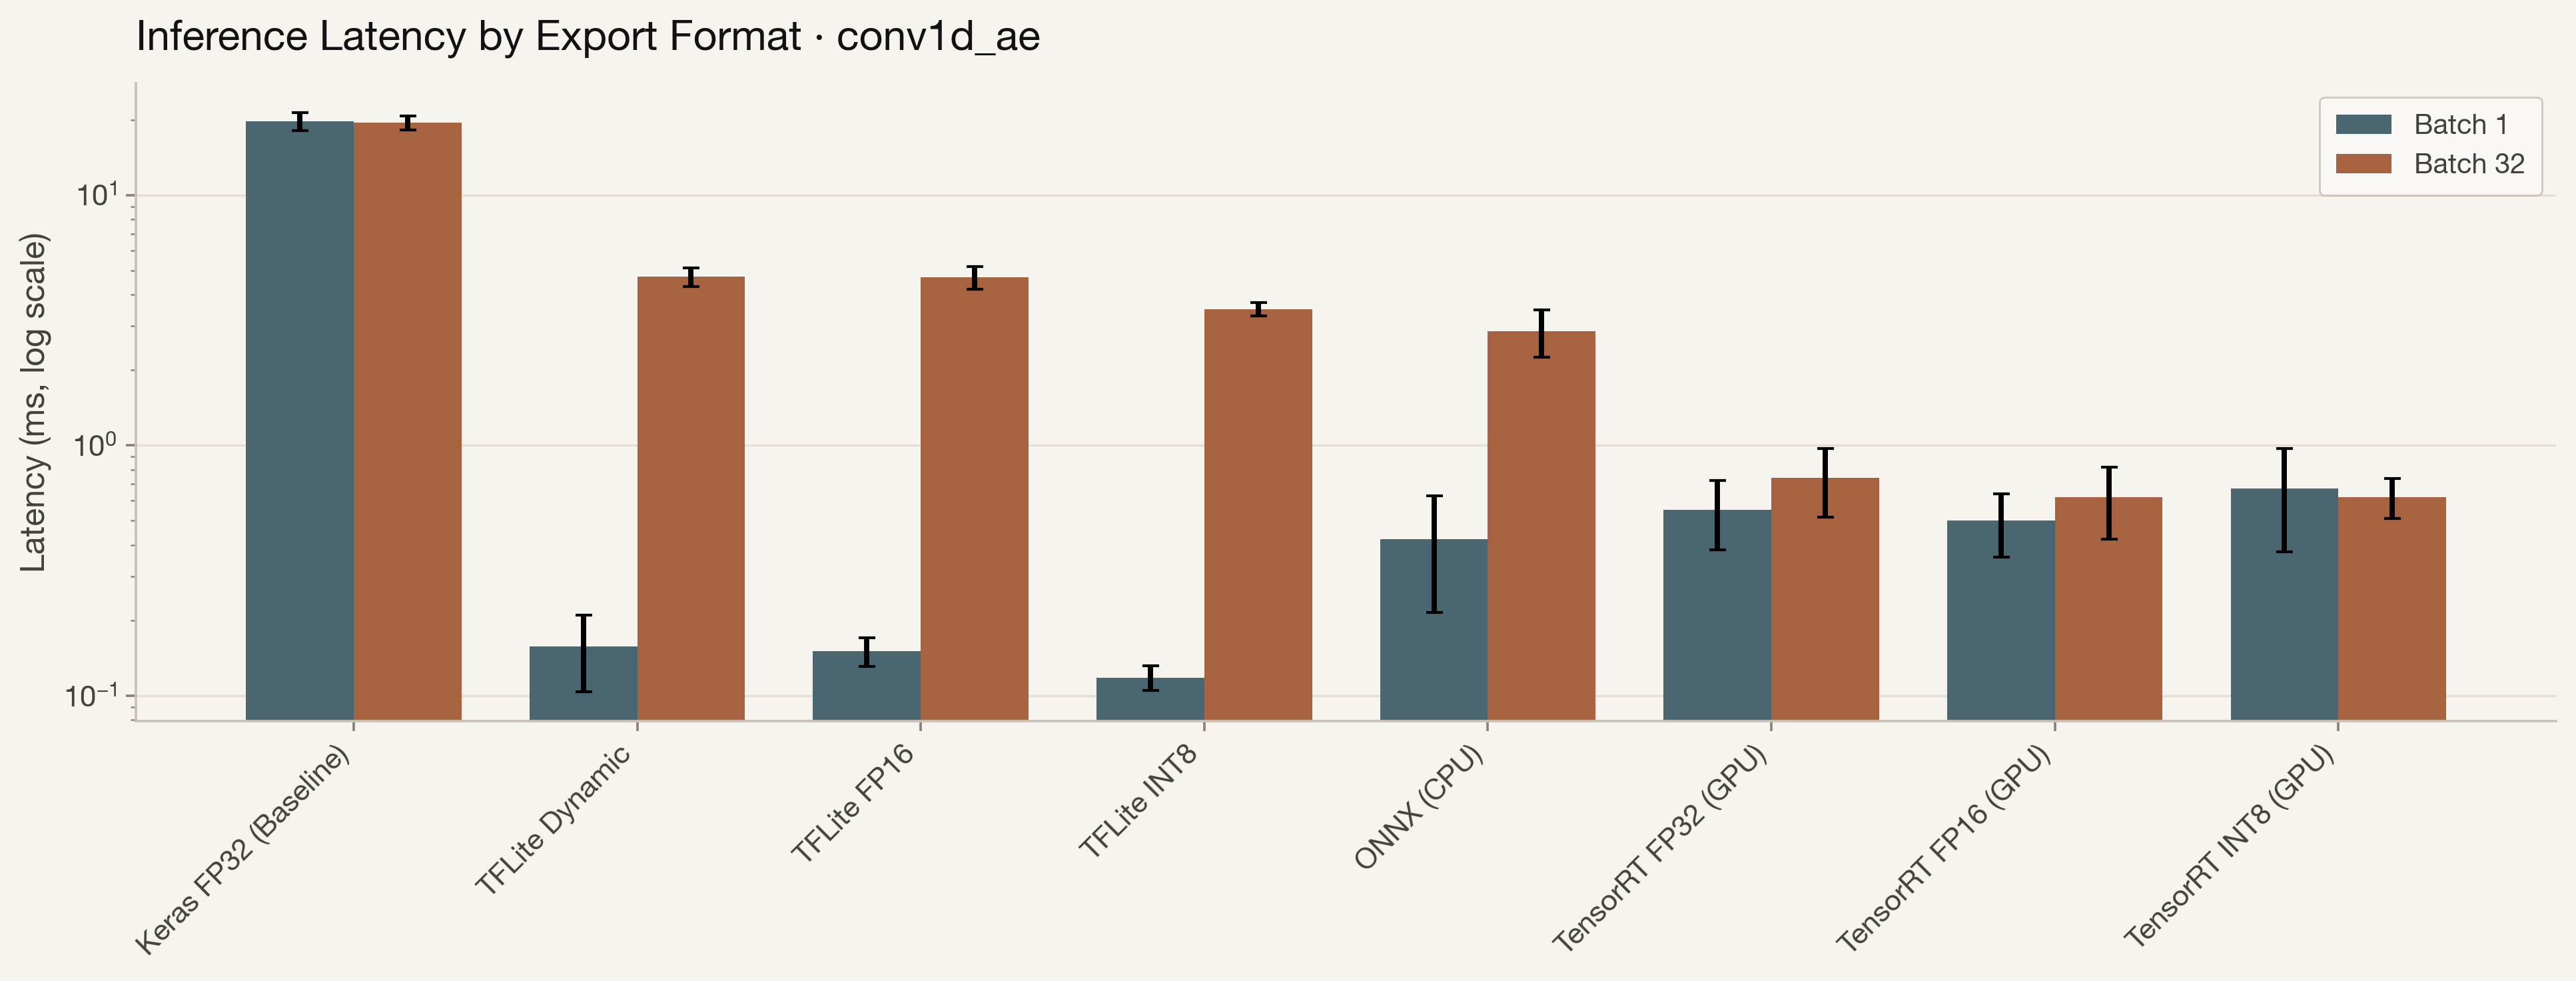
\includegraphics[width=0.48\textwidth]{deploy_latency_conv1d_ae.png}\hfill
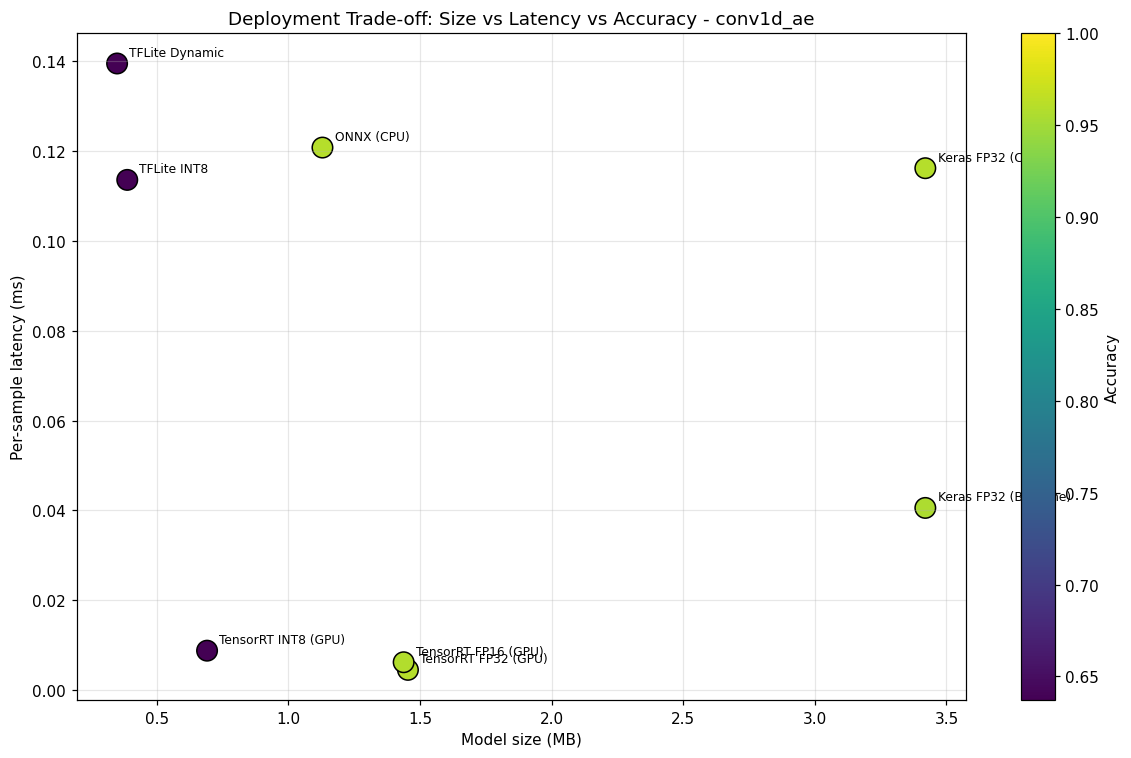
\includegraphics[width=0.48\textwidth]{deploy_tradeoff_conv1d_ae.png}
\caption{RTX 4070 interim platform: (left) per-format latency, log scale; (right)
latency-vs-ROC-AUC Pareto frontier. \realnote}
\label{fig:rtx-latency-tradeoff}
\end{figure}

\begin{figure}[ht]
\centering
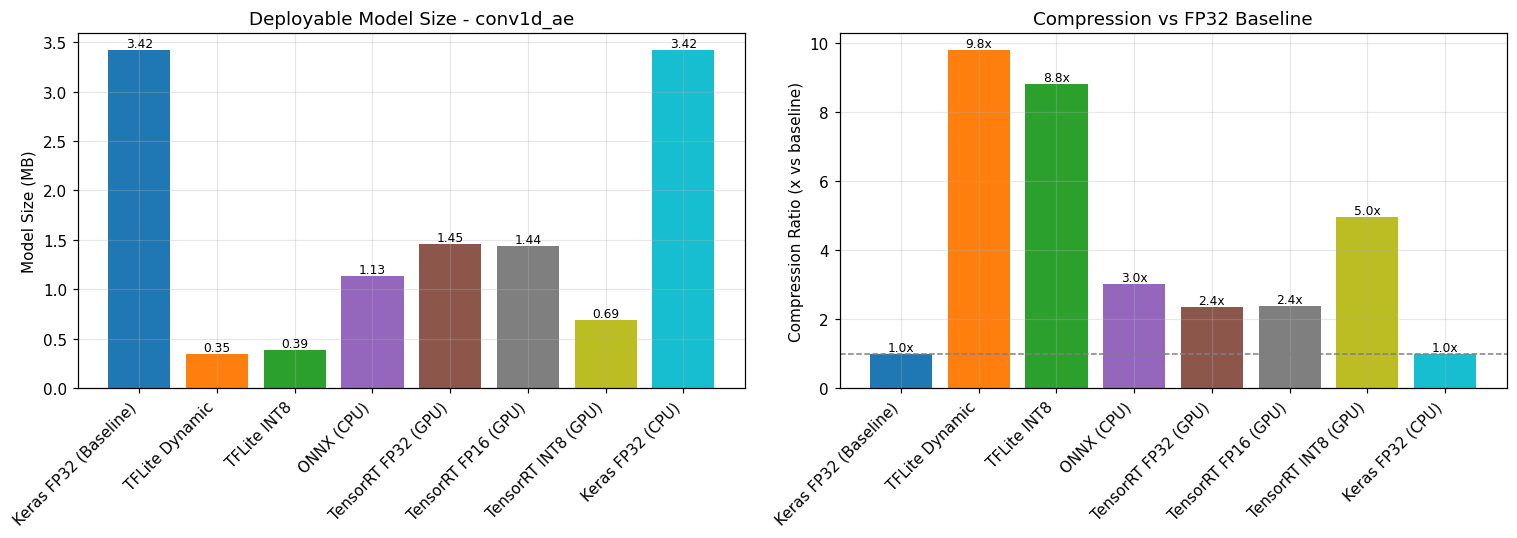
\includegraphics[width=0.7\textwidth]{deploy_model_size_conv1d_ae.png}
\caption{RTX 4070 interim platform: serialized model size across export formats. \realnote}
\label{fig:rtx-model-size}
\end{figure}

\subsection{Cross-hardware edge comparison: Jetson Nano vs.\ Xilinx ZCU102/ZCU104}
\label{sec:results-edge}

\begin{table}[ht]
\centering
\caption{Cross-hardware latency and memory, best available format per platform, batch-1. \mocknote}
\label{tab:edge-latency}
\begin{tabular}{@{}lcccc@{}}
\toprule
Platform & Format & Latency (ms) & Peak RAM/on-chip mem. (MB) & Model size (MB) \\
\midrule
RTX 4070 (interim, for reference) & TensorRT FP16 & 0.499 & --- & 1.44 \\
Jetson Nano & TensorRT [MOCK] & [MOCK] & [MOCK] & [MOCK] \\
Xilinx ZCU102 & Vitis AI INT8 (DPU) & [MOCK] & [MOCK] & [MOCK] \\
Xilinx ZCU104 & Vitis AI INT8 (DPU) & [MOCK] & [MOCK] & [MOCK] \\
\bottomrule
\end{tabular}
\end{table}

\begin{table}[ht]
\centering
\caption{Cross-hardware classification fidelity retention relative to the Keras FP32 baseline. \mocknote}
\label{tab:edge-fidelity}
\begin{tabular}{@{}lccccc@{}}
\toprule
Platform & Format & Accuracy & F1 & ROC-AUC & $\Delta$ ROC-AUC vs.\ FP32 \\
\midrule
Jetson Nano & TensorRT FP16 & [MOCK] & [MOCK] & [MOCK] & [MOCK] \\
Jetson Nano & TensorRT INT8 & [MOCK] & [MOCK] & [MOCK] & [MOCK] \\
Xilinx ZCU102 & Vitis AI INT8 & [MOCK] & [MOCK] & [MOCK] & [MOCK] \\
Xilinx ZCU104 & Vitis AI INT8 & [MOCK] & [MOCK] & [MOCK] & [MOCK] \\
\bottomrule
\end{tabular}
\end{table}

\begin{table}[ht]
\centering
\caption{Power and energy per inference (new metric, not yet instrumented). \mocknote}
\label{tab:edge-power}
\begin{tabular}{@{}lccc@{}}
\toprule
Platform & Avg.\ power (W) & Energy/inference (mJ) & Throughput per watt (inf/s/W) \\
\midrule
Jetson Nano & [MOCK] & [MOCK] & [MOCK] \\
Xilinx ZCU102 & [MOCK] & [MOCK] & [MOCK] \\
Xilinx ZCU104 & [MOCK] & [MOCK] & [MOCK] \\
\bottomrule
\end{tabular}
\end{table}

\figureplaceholder{edge-latency-bars}{Per-platform batch-1 latency, best format per
platform, log scale (RTX interim, Jetson Nano, Xilinx ZCU102/ZCU104).}

\figureplaceholder{edge-pareto}{Latency vs.\ ROC-AUC Pareto frontier across all
platform/format combinations, extending Figure~\ref{fig:rtx-latency-tradeoff} (right panel) with
the edge targets.}

\figureplaceholder{edge-throughput-per-watt}{Throughput per watt across platforms,
highlighting the expected GPU-embedded/FPGA-embedded power--performance trade-off.}

\section{Discussion}
\label{sec:discussion}

\textit{[Templated --- to be written once Tables~\ref{tab:edge-latency}--\ref{tab:edge-power}
contain real numbers; see Section~\ref{sec:reproducibility}.]} The discussion should
address: (i) whether Jetson Nano's software-programmable TensorRT path reaches
sub-millisecond batch-1 latency at edge power levels (5/10 W) comparable to the
workstation-GPU result in Section~\ref{sec:results-rtx}, or whether its far smaller
Maxwell GPU (128 vs.\ 5888 CUDA cores) pushes latency back toward the millisecond
range; (ii) whether the Xilinx DPU's statically compiled dataflow execution yields more
deterministic (lower-variance) latency than either GPU path, at the cost of the
INT8-only precision restriction and the qualitatively different, ahead-of-time
compilation workflow; (iii) which platform wins on throughput-per-watt
(Table~\ref{tab:edge-power}) and whether that ranking changes under a strict power
budget (e.g., battery-powered or thermally constrained deployments) versus a
performance-first budget; (iv) practical deployment guidance (development effort,
toolchain maturity, recompilation cost on model updates) that a purely numeric
comparison would miss.

\section{Conclusion and Future Work}
\label{sec:conclusion}

This paper presented a uniform quantization and multi-backend export pipeline for a
self-supervised power-converter anomaly detector and, building on an already-validated
workstation-GPU reference measurement (sub-millisecond batch-1 latency at
near-lossless fidelity via TensorRT FP16), scoped a head-to-head GPU-embedded (Jetson
Nano) vs.\ FPGA-embedded (Xilinx Zynq UltraScale+) deployment comparison. The
cross-hardware results in Section~\ref{sec:results-edge} are currently placeholders; the
immediate next step is executing the benchmarking campaign of
Section~\ref{sec:reproducibility} on physical Jetson Nano and ZCU102/ZCU104 hardware.
Beyond that, future work includes: extending the cross-hardware study to the remaining
six architectures (Section~\ref{sec:background}) including the physics-informed CARLA
model from the companion MMAS submission; implementing the power/energy instrumentation
described in Section~\ref{sec:methodology}; and exploring linear-complexity state-space
encoders~\cite{gu2023mamba} as a further latency reduction on both edge targets.

\section{Reproducibility}
\label{sec:reproducibility}

\textbf{Optimize (quantize/compile) a model for a given target:}
\begin{verbatim}
python -m src.deployment_optimization \
  --model-dir experiments/conv1d_ae \
  --data-dir data/buck/buck_data \
  --vitis-target zcu102        # or zcu104 for the second Xilinx target
\end{verbatim}
\textbf{Benchmark the converted formats:}
\begin{verbatim}
python -m src.deployment_evaluation \
  --model-dir experiments/conv1d_ae \
  --data-dir data/buck/buck_data
\end{verbatim}
On \textbf{Jetson Nano}, both commands are run on-device (JetPack ships its own
TensorRT/CUDA build; engines must be re-serialized locally and do not carry over from
the RTX host) -- no pipeline code changes are anticipated. On \textbf{Xilinx
ZCU102/ZCU104}, the Vitis AI INT8 quantize+compile step is run on a host with the Vitis
AI Docker toolchain, and the resulting \texttt{.xmodel} is copied to the board and
executed via the \texttt{pynq-dpu} runtime. Power/energy instrumentation
(Table~\ref{tab:edge-power}) is not yet implemented and is tracked as follow-up work.
Full details and current status are maintained in the project's research plan,
\texttt{papers/PLAN.md}, Section~4.3.

\section*{Data Availability Statement}
Benchmarking scripts and (upon publication) raw timing logs for every platform/format
combination will be made publicly available alongside the companion MMAS submission's
dataset release.

\section*{Conflict of Interest Statement}
\textit{[TODO --- to be completed by the authors; assumed ``The authors declare no
conflict of interest'' pending confirmation.]}

\section*{Acknowledgements}
\textit{[TODO --- funding sources and institutional acknowledgements to be added by the
authors.]}

\bibliographystyle{unsrt}
\bibliography{../shared/references}

\end{document}
